\paragraph*{Personalizzazione} I clienti possono essere disposti a pagare per
avere un prodotto esattamente ritagliato sulle loro esigenze. Per esempio, la
sartoria fa le camicie su misura: il loro costo è superiore\footnote{In quanto,
rispetto a un'economia di scala dove a fronte di un investimento iniziale
maggiore per i macchinari si ha la possibilità di avere una maggiore
produzione, abbassando i costi del prodotto finale, rispetto al prodotto
``fatto a mano''.}, come il tempo stesso di produzione della camicia, che
è più lungo poiché deve essere prodotto manualmente. Qui esistono due tipologie
di clienti: c'è chi vuole la gratificazione immediata dopo l'acquisto e chi
invece preferisce spendere del tempo nella personalizzazione e nell'attesa ma
ricevere un prodotto unico.
Negli anni recenti si parla spesso di personalizzazione di massa, o
\textit{mass customization}, e di co-creazione. La prima permette ai clienti di
scegliere tra diverse opzioni di customizzazione che possono essere combinate
tra loro. Un esempio tipico in questo caso sono le automobili. Nella seconda,
invece, sono gli utenti stessi che in qualche modo modificano il percorso
evolutivo di un prodotto, ed un esempio in questo caso è la creazione di alcuni
videogiochi.

\paragraph*{Supporto} Il valore può venire creato semplicemente aiutando il
cliente ad ottenere un determinato risultato, facendo si che un certo lavoro
venga portato a termine. Per esempio le aziende che creano prodotti
open-source e offrono supporto all'utilizzo di essi (ad esempio Red Hat) o
appunto chi consulenze. Spesso, in quest'ultimo caso la
prima consulenza è un lavoro ``in perdita'' o con bassissima rendita, ma le
consulenze successive sono molto più semplici. Ciò è dovuto al fatto che la
prima collaborazione richiede uno studio approfondito del contesto aziendale.
Un esempio può essere una consulenza legale: può essere che l'azienda possa, da
sola, creare i propri contratti, ma ciò richiederebbe uno sforzo maggiore e
potrebbe comportare degli errori. Un consulente legale la prima volta dovrà
capire le esigenze dell'azienda ma le volte successive il suo lavoro sarà
agevolato dallo studio iniziale.

\paragraph*{Design} Un prodotto può venire scelto perché si differenzia per un
design superiore. Questa è una delle value proposition centrali della moda
(insieme al brand), macchine (possibilmente insieme al brand) e ultimamente
anche dell'elettronica (vedi Apple).

\paragraph*{Brand/Status} A volte il puro utilizzo e l'ostentazione di un
determinato prodotto può creare \textbf{valore} per un cliente (esempio
Ferrari). È importante notare che non solo i prodotti di lusso vengono scelti
in base al brand, ma ciò vale anche per alcuni prodotti di massa come Converse.

\paragraph*{Prezzo} Offrire il medesimo servizio ad un costo più basso rispetto
alla concorrenza è un modo usuale di creare valore, come ad esempio Ikea,
Ryanair, ecc\dots Lavorare sul prezzo è una leva molto forte, ed impatta 
fortemente su tutto il resto del business model: è molto complicato offrire lo
stesso livello qualitativo di un prodotto della concorrenza offerto a prezzo
maggiore. È necessario, infatti, capire dov'è possibile abbassare la qualità
del prodotto su caratteristiche che non sono considerate importanti o sensibili
per il cliente e investire invece sulle altre.

\paragraph*{Riduzione dei costi} Aiutare i clienti a ridurre i loro costi
operativi (come ad esempio le soluzioni SaaS\footnote{Software As A Service}). 
Ciò può far sì che sia necessario fare un investimento iniziale maggiore,
che finisce per comportare una riduzione dei costi a lungo termine.\\[0.3cm]

La value proposition che interessano di più la fedeltà del cliente sono per
esempio quelle associate al \textbf{brand} e al \textbf{supporto}, il quale
prevede delle dinamiche di vendita che solitamente richiedono dei tempi lunghi,
nel quale è necessario convincere il cliente della propria affidabilità. Non
influisce sulla fedeltà invece una value proposition incentrata sul prezzo.

\begin{figure}[t]
 \centering
 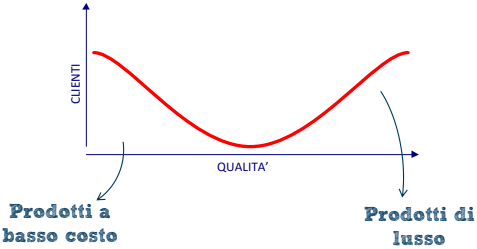
\includegraphics[scale=0.65]{prices_distribution}
 \caption[Distribuzione dei prezzi]{Distribuzione delle fasce di prezzo per i 
prodotti: com'è possibile notare al giorno d'oggi i prodotti tendono ad avere 
costi polarizzati, ovvero o sono molto costosi o non lo sono affatto. La fascia 
di prodotti a prezzo ``medio'' sta lentamente scomparendo.}
 \label{fig:vp:pd}
\end{figure}

\noindent In passato i clienti cercavano il miglior rapporto qualità/prezzo. In
anni più recenti si è visto un fenomeno molto forte, detto
\textbf{polarizzazione} che ha portato all'inversione di questa curva (come 
rappresentato in Figura~\ref{fig:vp:pd}) in quanto c'è stato uno spostamento 
verso gli estremi. Da un lato si ha una gamma di prodotti luxury, mentre 
dall'altro si presentano, per esempio, il proliferare di compagnie low cost, o 
di discount.

Questo a causa di un forte cambiamento della realtà di consumo dei singoli.
Riflettendoci attentamente, ciascuno di noi oggi è molto più selettivo
(rispetto al passato) in quanto ognuno di noi ha le idee più chiare su dove uno
vuole spendere i suoi soldi o meno. È quindi chiaro che in alcune categorie si
preferisca l'uso di prodotto low-cost in alcuni settori, mentre in altri si
spende molto di più per prodotti luxury. Le leve per questo fenomeno sono
molte, ma principalmente tutto ciò è dovuto alla crisi economica, che ha
ridotto le capacità di acquisto medio, e dall'altra la diffusione
dell'informazione, che oggi permette di informarsi molto più facilmente su un
prodotto.

Quindi, oggi come oggi, posizionare i prodotti in una fascia media è
pericolosissimo, ed è meglio effettuare una polarizzazione verso gli estremi.
